\subsection{Local Spatial Transformations and Correlation}\label{sec:local-spatial-transformations-and-correlation}

\subsubsection{Local Neighbourhoods}\label{sec:local-neighbourhoods}

So far we have represented an image as a tensor:
\begin{equation*}
    I \in \mathbb{R}^{R \times C \times 3}
\end{equation*}
Where every pixel has RGB values. But, \textbf{\emph{how can we transform an image?}} More specifically, \textbf{\emph{how can we compute a new image from an existing one?}} The answer introduced in this sections is to use \textbf{local spatial transformations}.

\highspace
\begin{flushleft}
    \textcolor{Green3}{\faIcon{balance-scale} \textbf{Global vs Local Transformations}}
\end{flushleft}
Suppose we want to modify an image. There are two possible philosophies:
\begin{itemize}
    \item \important{Global Transformations}. Each output pixel depends on \textbf{every pixel} in the image. Obviously, this is very expensive to compute. For example, if we want to compute the average color of an image, we need to look at every pixel in the image.
    \item \important{Local Transformations}. Instead of looking at every pixel in the image, the output pixel only depends on a \textbf{small neighborhood} around it. Everything outside the square is ignored. This is much more efficient and, more importantly, \textbf{it matches the structure of natural images}. Because nearby pixels are usually much more related than distant pixels.
\end{itemize}

\highspace
\begin{flushleft}
    \textcolor{Green3}{\faIcon{question-circle} \textbf{What is a Neighbourhood? And why is it called Local?}}
\end{flushleft}
A \definition{neighbourhood} $U$ is a \textbf{small window centered on the pixel we are processing}. The central pixel is denoted as $(r,c)$, where $r$ is the row and $c$ is the column of the pixel. The neighbourhood is usually a square of size $k \times k$, where $k$ is an odd number. The reason for using an odd number is that it allows us to have a single central pixel with an equal number of pixels on each side. For example, a $3 \times 3$ neighbourhood has one central pixel and 8 surrounding pixels.

\highspace
Again, only these pixels are used to compute the output pixel. \hl{Everything outside the square is ignored.} This is why it is called a \textbf{local} transformation.

\highspace
\textcolor{Green3}{\faIcon{tools} \textbf{Transformation Function $T_U$.}} Up to now we have only defined the \textbf{local neighbourhood} $U_{r,c}$. Now suppose we want to blur the image, sharpen it, detect edges, remove noise, or perform any other image processing task. All these operations create \textbf{another image} (output) $G$ from the original image $I$. But \emph{\textbf{how should the value of one output pixel $G(r, c)$ be computed from the input image $I$?}} The answer is that we need to look only at the neighbourhood around $\left(r,c\right)$, then apply some rule $T_U$ to compute the output pixel.

\highspace
In other words, we can define a \textbf{transformation} $T_U$ as a \textbf{function} that takes as input a neighbourhood $U_{r,c}$ and produces as output a single pixel value $G(r,c)$:
\begin{equation*}
    G(r,c) = T_U\left(I\right)\left(r,c\right)
\end{equation*}
The output pixel at $\left(r,c\right)$ is obtained by applying the transformation $T_U$ to the local neighbourhood centered at $\left(r,c\right)$ in the original input image $I$.

\begin{figure}[!htp]
    \centering
    \resizebox{\textwidth}{!}{
        \begin{tikzpicture}[
            >=Latex,
            every node/.style={font=\small},
            pixel/.style={draw=gray!50, line width=0.4pt, fill=gray!10},
            centerpix/.style={draw=black, line width=1pt, fill=orange!45},
            neighbox/.style={draw=blue!80, dashed, line width=0.9pt}
        ]

            % Parameters
            \def\s{0.75}      % cell size
            \def\N{7}         % grid size

            % =========================================================
            % Input image I
            % =========================================================

            % Input grid
            \foreach \i in {0,...,6}{
                \foreach \j in {0,...,6}{
                    \path[pixel] (\j*\s,-\i*\s) rectangle ++(\s,-\s);
                }
            }

            % Center pixel coordinates in the grid
            \def\cx{3}
            \def\cy{3}

            % 3x3 neighbourhood around (r,c)
            \fill[blue!12] ({(\cx-1)*\s},{-(\cy-1)*\s})
                rectangle ++({3*\s},{-3*\s});

            % Redraw grid lines over the neighbourhood
            \foreach \i in {0,...,6}{
                \foreach \j in {0,...,6}{
                    \draw[gray!50, line width=0.4pt]
                    (\j*\s,-\i*\s) rectangle ++(\s,-\s);
                }
            }

            % Center pixel
            \path[centerpix] (\cx*\s,-\cy*\s) rectangle ++(\s,-\s);

            % Dashed neighbourhood boundary
            \draw[neighbox]
                ({(\cx-1)*\s},{-(\cy-1)*\s})
                rectangle ++({3*\s},{-3*\s});

            % Labels on input image
            \node[font=\normalsize] at ({3.5*\s},0.9) {Input image $I$};
            \node[text=blue!80!black] at ({3.5*\s},{-(\cy-1)*\s + 0.35}) {$U_{r,c}$};
            \node at ({(\cx+0.5)*\s},{-(\cy+0.5)*\s}) {$(r,c)$};

            % =========================================================
            % Transformation arrow
            % =========================================================

            \draw[->, line width=0.9pt]
                ({7.4*\s},{-3.5*\s})
                -- ({10.0*\s},{-3.5*\s});

            \node[above] at ({8.7*\s},{-3.5*\s}) {$T_U$};

            % =========================================================
            % Output image G
            % =========================================================

            % Output grid shifted to the right
            \def\xshift{10.6}

            \foreach \i in {0,...,6}{
                \foreach \j in {0,...,6}{
                    \path[pixel] ({\xshift*\s+\j*\s},{-\i*\s})
                    rectangle ++(\s,-\s);
                }
            }

            % Highlight output pixel G(r,c)
            \path[centerpix]
                ({\xshift*\s+\cx*\s},{-\cy*\s})
                rectangle ++(\s,-\s);

            % Output labels
            \node[font=\normalsize] at ({\xshift*\s+3.5*\s},0.9) {Output image $G$};

            \node[right=0.25cm] at ({\xshift*\s+(\cx+1)*\s},{-(\cy+0.5)*\s})
                {$G(r,c)$};

        \end{tikzpicture}
    }
    \caption{A local transformation $T_U$ that computes the output pixel $G(r,c)$ from the input image $I$ using only the local neighbourhood $U_{r,c}$.}
\end{figure}

\highspace
\textcolor{Green3}{\faIcon{question-circle} \textbf{How is a Neighbourhood described?}} Suppose we are currently computing the output pixel at $\left(r,c\right)$. The neighbourhood $U_{r,c}$ is a square of size $k \times k$ centered at $\left(r,c\right)$. For example, if $k=3$, the neighbourhood is:
\begin{equation*}
    U_{r,c} = \begin{bmatrix}
        I(r-1,c-1) & I(r-1,c) & I(r-1,c+1) \\
        I(r,c-1) & I(r,c) & I(r,c+1) \\
        I(r+1,c-1) & I(r+1,c) & I(r+1,c+1)
    \end{bmatrix}
\end{equation*}
The neighbourhood is \textbf{not described by absolute coordinates}, but rather by \textbf{offsets from the center}. Thus, we introduce the following notation:
\begin{equation*}
    I\left(r + u, c + v\right), \quad \left(u,v\right) \in U
\end{equation*}
Where $r,c$ are the \textbf{absolute position} of the current pixel, and $u,v$ are the \textbf{relative displacement} from that pixel. For example, in a $3 \times 3$ neighbourhood, the offsets are:
\begin{align*}
    U &= \left\{(-1,-1), (-1,0), (-1,1), (0,-1), (0,0), (0,1), (1,-1), (1,0), (1,1)\right\} \\
    &\to \begin{bmatrix}
        (-1,-1) & (-1,0) & (-1,1) \\
        (0,-1) & (0,0) & (0,1) \\
        (1,-1) & (1,0) & (1,1)
    \end{bmatrix}
\end{align*}
The central pixel is at offset $(0,0)$, but $\left(r,c\right)$ can be any pixel in the image, such as $\left(r,c\right) = \left(20,50\right)$. Thus:
\begin{equation*}
    I\left(20 + 0, 50 + 0\right) = I(20,50) \quad u,v = (0,0) \in U
\end{equation*}

\newpage

\begin{figure}[!htp]
    \centering
    \tikzsetnextfilename{local-neighbourhoods}
    \begin{tikzpicture}[
        cell/.style={
            draw=gray!55,
            minimum size=1.25cm,
            inner sep=0pt
        },
        neigh/.style={
            fill=green!15
        },
        center/.style={
            fill=green!45
        },
        labelcell/.style={
            font=\scriptsize,
            align=center
        },
        arrow/.style={
            ->,
            thick,
            >=stealth
        }
    ]

    % Cell size
    \def\s{1.25}

    % Draw 5x5 grid
    \foreach \r in {0,...,4} {
        \foreach \c in {0,...,4} {

            \pgfmathsetmacro{\x}{\c*\s}
            \pgfmathsetmacro{\y}{-\r*\s}

            % Highlight 3x3 neighbourhood
            \ifnum\r>0
                \ifnum\r<4
                    \ifnum\c>0
                        \ifnum\c<4
                            \node[cell, neigh] at (\x,\y) {};
                        \else
                            \node[cell] at (\x,\y) {};
                        \fi
                    \else
                        \node[cell] at (\x,\y) {};
                    \fi
                \else
                    \node[cell] at (\x,\y) {};
                \fi
            \else
                \node[cell] at (\x,\y) {};
            \fi
        }
    }

    % Center pixel
    \node[cell, center] at (2*\s,-2*\s) {};
    \node[labelcell] at (2*\s,-2*\s) {$I(r,c)$};

    % Displacement labels
    \node[labelcell] at (1*\s,-1*\s) {$(-1,-1)$};
    \node[labelcell] at (2*\s,-1*\s) {$(-1,0)$};
    \node[labelcell] at (3*\s,-1*\s) {$(-1,1)$};

    \node[labelcell] at (1*\s,-2*\s) {$(0,-1)$};
    \node[labelcell] at (3*\s,-2*\s) {$(0,1)$};

    \node[labelcell] at (1*\s,-3*\s) {$(1,-1)$};
    \node[labelcell] at (2*\s,-3*\s) {$(1,0)$};
    \node[labelcell] at (3*\s,-3*\s) {$(1,1)$};

    % Dashed border around neighbourhood
    \draw[dashed, very thick, green!60!black]
        ($(1*\s,-1*\s)+(-0.625,0.625)$)
        rectangle
        ($(3*\s,-3*\s)+(0.625,-0.625)$);

    % Arrow from center to upper-right neighbour
    \draw[arrow, orange!85!black]
        ($(2*\s,-2*\s)+(0.15,0.15)$)
        --
        ($(3*\s,-1*\s)+(-0.20,-0.20)$);

    % Arrow label outside the grid
    \node[
        orange!85!black,
        font=\scriptsize,
        anchor=west
    ] at ($(3*\s,-1*\s)+(0.75,-0.15)$)
        {$u=-1,\ v=1$};

    % Axis arrows
    \draw[arrow] ($(0,0.9)$) -- ($(1.4,0.9)$)
        node[midway, above] {columns $c$};

    \draw[arrow] ($(-0.9,-0.2)$) -- ($(-0.9,-1.6)$)
        node[midway, left] {rows $r$};

    \end{tikzpicture}
    \caption{A local neighbourhood $U_{r,c}$ represented as a set of displacement vectors $(u,v)$ around the central pixel $(r,c)$.}
    \label{fig:local-neighbourhoods}
\end{figure}

\begin{flushleft}
    \textcolor{Green3}{\faIcon{question-circle} \textbf{How do we transform the entire image?}}
\end{flushleft}
We have defined how to compute a single output pixel $G(r,c)$ from the input image $I$ using the local neighbourhood $U_{r,c}$. But, \textbf{\emph{how do we compute the entire output image $G$?}} The answer is that we need to \textbf{move the neighbourhood} to the next pixel in the image, and repeat the process for every pixel in the image. This is done by iterating over all pixels $(r,c)$ in the input image $I$, applying the transformation $T_U$ to each local neighbourhood $U_{r,c}$, and storing the result in the corresponding output pixel $G(r,c)$. This movement of the neighbourhood is called the \definition{Sliding Window}.

\begin{figure}[!htp]
    \centering
    \tikzsetnextfilename{sliding-window-mechanism}
    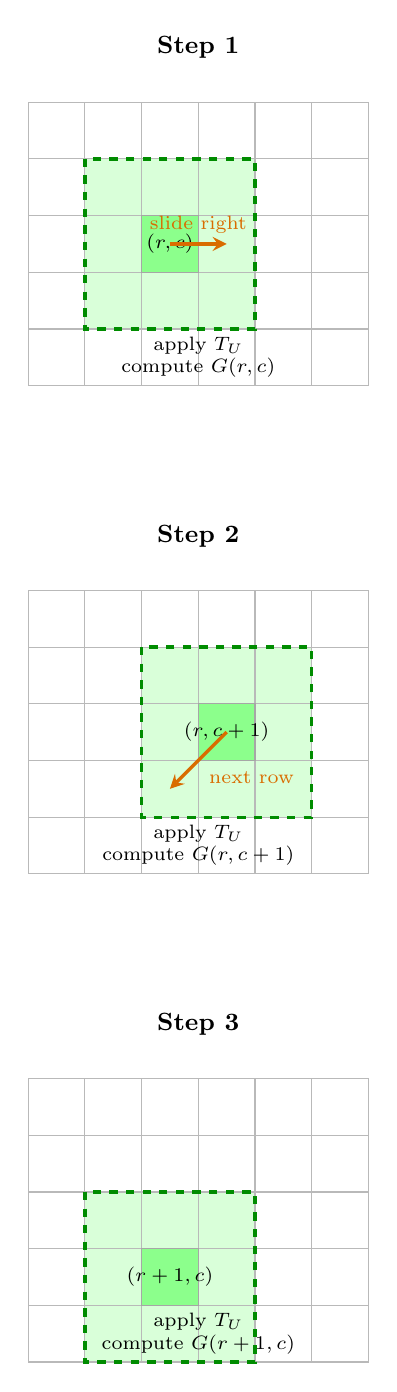
\begin{tikzpicture}[
        cell/.style={
            draw=gray!55,
            minimum size=0.72cm,
            inner sep=0pt
        },
        windowcell/.style={
            fill=green!15,
            draw=gray!55,
            minimum size=0.72cm,
            inner sep=0pt
        },
        centerpixel/.style={
            fill=green!45,
            draw=gray!70,
            minimum size=0.72cm,
            inner sep=0pt
        },
        title/.style={
            font=\bfseries\small
        },
        smalllabel/.style={
            font=\scriptsize,
            align=center
        },
        movearrow/.style={
            ->,
            very thick,
            orange!85!black,
            >=stealth
        }
    ]

    \def\s{0.72}

    % ---------------------------------------------------------
    % Draw one panel
    % Arguments:
    % #1 = y shift
    % #2 = title
    % #3 = center row
    % #4 = center column
    % #5 = center label
    % #6 = output label
    % ---------------------------------------------------------
    \newcommand{\drawPanel}[6]{
    \begin{scope}[shift={(0,#1)}]

        % Title
        \node[title] at ({2.5*\s}, {1.05}) {#2};

        % Base 5x6 grid
        \foreach \r in {0,...,4} {
            \foreach \c in {0,...,5} {
                \node[cell] at ({\c*\s}, {-\r*\s}) {};
            }
        }

        % Highlight 3x3 neighbourhood
        \foreach \dr in {-1,0,1} {
            \foreach \dc in {-1,0,1} {
                \pgfmathtruncatemacro{\rr}{#3+\dr}
                \pgfmathtruncatemacro{\cc}{#4+\dc}
                \node[windowcell] at ({\cc*\s}, {-\rr*\s}) {};
            }
        }

        % Center pixel
        \node[centerpixel] at ({#4*\s}, {-#3*\s}) {};
        \node[smalllabel] at ({#4*\s}, {-#3*\s}) {#5};

        % Dashed border around window
        \draw[
            dashed,
            very thick,
            green!55!black
        ]
        ({(#4-1.5)*\s}, {(-#3+1.5)*\s})
        rectangle
        ({(#4+1.5)*\s}, {(-#3-1.5)*\s});

        % Output label, placed far below the grid
        \node[smalllabel] at ({2.5*\s}, {-4.0*\s}) {
            apply $T_U$\\%[-1mm]
            compute #6
        };

    \end{scope}
    }

    % ---------------------------------------------------------
    % Panels
    % ---------------------------------------------------------
    \drawPanel{0}{Step 1}{2}{2}{$(r,c)$}{$G(r,c)$}

    \drawPanel{-6.2}{Step 2}{2}{3}{$(r,c+1)$}{$G(r,c+1)$}

    \drawPanel{-12.4}{Step 3}{3}{2}{$(r+1,c)$}{$G(r+1,c)$}

    % ---------------------------------------------------------
    % Precise movement arrows INSIDE the grids
    % ---------------------------------------------------------

    % Step 1: slide right from (r,c) to (r,c+1)
    \draw[movearrow]
        ({2*\s}, {-2*\s})
        --
        ({3*\s}, {-2*\s})
        node[midway, above, font=\scriptsize, orange!85!black]
        {slide right};

    % Step 2: move to next row
    \begin{scope}[shift={(0,-6.2)}]
    \draw[movearrow]
        ({3*\s}, {-2*\s})
        --
        ({2*\s}, {-3*\s})
        node[midway, below right, font=\scriptsize, orange!85!black]
        {next row};
    \end{scope}

    \end{tikzpicture}
    \caption{Sliding window mechanism. The same local transformation $T_U$ is applied at different spatial positions to compute the corresponding output pixels.}
    \label{fig:sliding-window-mechanism}
\end{figure}